\documentclass[a4paper]{article}
\usepackage[top=1in,bottom=1in,left=1in,right=1in]{geometry}
\usepackage{times}
\usepackage{amssymb}
\usepackage{mathtools}	% pulls in amsmath
	\mathtoolsset{centercolon}
\usepackage{tikz}
	\usetikzlibrary{automata}
	\usepackage{tikz-qtree}
\usepackage{mathpartir}
\usepackage{amsthm}
\usepackage{amsxtra}
\usepackage{algorithm}
\usepackage{algpseudocode}
\usepackage{semantic}
	\reservestyle{\declarevars}{\texttt}
	\reservestyle{\declareops}{\texttt}
	\reservestyle{\declarestates}{\text}
\usepackage{color}
\usepackage{listings}
\usepackage{mathtools}
\usepackage[shortlabels]{enumitem}
\usepackage{graphicx}	% for pdf image
\usepackage{pgfplots}
\pgfplotsset{width=7cm}

\newtheorem{theorem}{Theorem}

\newtheorem{myexample}{\textbf{Example}}
\newtheorem{mylemma}{\textbf{Lemma}}
\newtheorem{myproof}{\textbf{Proof}}
\newtheorem{myinvariant}{\textbf{Invariant}}
\newtheorem{mytheorem}{\textbf{Theorem}}
\newtheorem{mycorollary}{\textbf{Corollary}}
\newtheorem{myapproach}{Approach}
\newtheorem{myproperty}{Property}
\newtheorem{mydefinition}{Definition}

\newtheorem{mycase}{Case}

\lstset{ %
  backgroundcolor=\color{white},   % choose the background color; you must add \usepackage{color} or \usepackage{xcolor}
  basicstyle=\small,        % the size of the fonts that are used for the code
  breakatwhitespace=false,         % sets if automatic breaks should only happen at whitespace
  breaklines=true,                 % sets automatic line breaking
  captionpos=b,                    % sets the caption-position to bottom
  commentstyle=,    % comment style
  deletekeywords={...},            % if you want to delete keywords from the given language
  escapeinside={\%*}{*)},          % if you want to add LaTeX within your code
  extendedchars=true,              % lets you use non-ASCII characters; for 8-bits encodings only, does not work with UTF-8
 % frame=single,                    % adds a frame around the code
  keepspaces=true,                 % keeps spaces in text, useful for keeping indentation of code (possibly needs columns=flexible)
  columns=fullflexible,	% not monospace
  keywordstyle=,       % keyword style
  language=Octave,                 % the language of the code
  morekeywords={forall, to, else, then, end, and, or, assign, increment, decrement, jump, jump_if, store, *, +},            % if you want to add more keywords to the set
  numbers=left,                    % where to put the line-numbers; possible values are (none, left, right)
  numbersep=5pt,                   % how far the line-numbers are from the code
  rulecolor=\color{black},         % if not set, the frame-color may be changed on line-breaks within not-black text (e.g. comments (green here))
  showspaces=false,                % show spaces everywhere adding particular underscores; it overrides 'showstringspaces'
  showstringspaces=false,          % underline spaces within strings only
  showtabs=false,                  % show tabs within strings adding particular underscores
  stepnumber=1,                    % the step between two line-numbers. If it's 1, each line will be numbered
  stringstyle=,     % string literal style
  tabsize=4,                       % sets default tabsize to 2 spaces
  title=\lstname,                  % show the filename of files included with \lstinputlisting; also try caption instead of title
  mathescape,
  belowskip=-\baselineskip,
}

\DeclareMathOperator{\prob}{prob}
\DeclareMathOperator{\dom}{dom}
\DeclareMathOperator{\rank}{rank}
\DeclareMathOperator{\key}{key}
\newcommand*{\floor}[1]{\left\lfloor{#1}\right\rfloor}
\newcommand*{\ceil}[1]{\left\lceil{#1}\right\rceil}
\newcommand{\any}{{\rule[-.2ex]{1ex}{.4pt}}}	% Less hideous than \_.
\newcommand{\RR}{\mathbb{R}}
\newcommand{\NN}{\mathbb{N}}
\newcommand{\ZZ}{\mathbb{Z}}
\newcommand{\RP}{\RR_{\ge 0}}
\newcommand*{\dave}[1]{{\color{red}\textbf{PDS: #1}}}
\newcommand{\ie}{\emph{i.e.,} }
\newcommand{\eg}{\emph{e.g.,} }
\usepackage{hyperref}
\newcommand*{\Sref}[1]{\hyperref[#1]{\S\ref*{#1}}}
\newcommand*{\figref}[1]{\hyperref[#1]{Figure~\ref*{#1}}}
\newcommand{\edge}{\longrightarrow}
\newcommand{\redge}{\longleftarrow}

\title{Exercise Sheet 11---Algorithms and Data Structures}
\author{Felipe Cerqueira \\ 2547787 \and David Swasey \\ 2542105}

\begin{document}

\maketitle

Tutorial time: Monday 14:00


\section*{Exercise 1 (10 pts)}

The polar angle of a point $p_1$ with respect to $p_0$ is the angle that the vector $p_1 - p_0$ forms in the usual polar coordinate system. For instance, the polar angle of $(3, 5)$ with respect to $(2, 4)$ is the angle of $(1, 1)$, which is 45 degrees, or $\pi/4$. The polar angle of $(3, 3
)$ with respect to $(2, 4)$ is the angle of $(1, -1)$, which is 315 degrees or $7\pi/4$. Design an $O(n \log n)$-algorithm that sorts a sequence of $n$ points $p_1, \ldots, p_n$ according to the polar angles with respect to a given origin $p_0$. Your algorithm should avoid computing the angles explicitly.

\paragraph{Answer.}

In order to compare the polar angle between two points $p_1$ and $p_2$, we just check whether one of the vectors is counter-clockwise with respect to the other, i.e., compute $CCW(p_0, p_1, p_2)$.

However, computing ${CCW}(\cdots)$ via cross product only is not sufficient. Since there are corner cases when the points are collinear and reside in different quadrants, we can use the following implementation instead.

Source: \url{http://www.mathcs.duq.edu/simon/Fall05/cs300notes3.html}

\begin{lstlisting}[mathescape]
${CCW}'(p_0,p_1,p_2)$
{
  dx1$\gets (x_1-x_0)$
  dy1 $\gets (y_1-y_0)$
  dx2 $\gets (x_2-x_0)$
  dy2 $\gets (y_2-y_0)$;
  if(dy1*dx2 < dy2*dx1) return 1;
  if(dy1*dx2 > dy2*dx1) return -1;
  if(dx1*dx2 < 0 || dy1*dy2 < 0) return -1;
  if(dx1*dx1 + dy1*dy1 >= dx2*dx2 + dy2*dy2)
    return 0;
  else
    return 1;
}
\end{lstlisting}




%\begin{figure}[h]
%\centering
%\begin{tikzpicture}
%\draw[style=help lines,step=0.5cm] (-3,-3) grid (3,3);

%    \draw[->,thick, color=blue] (-3.1,0) -- (3.1,0) node[anchor=west]{x};
%    \draw[->,thick] (0,-3.1) -- (0,3.1) node[anchor=south]{y};
    %
%    \foreach \x in {0,1,...,3} \draw [thick](\x cm,-2pt) -- (\x cm,2pt);
%    \foreach \y in {0,1,...,3} \draw [thick](-2pt,\y) -- (2pt,\y);
    
% \begin{scope}[color=red]
%    \filldraw (0,0) circle (0.08cm)  {} node[anchor=west,yshift=0.25cm, xshift=0.2cm] {CCW?};
%    \filldraw (2,1.5) circle (0.08cm) {} node[anchor=west,xshift=5pt] {2};
    %\filldraw (1.5,2) circle (0.08cm){} node[anchor=south,yshift=0.1cm] {3};
%    \filldraw (5,1) circle (0.08cm)  {} node[anchor=north,yshift=-0.1cm] {4};
%    \filldraw (3,5) circle (0.08cm) {} node[anchor=west,xshift=5pt] {5};
%\end{scope}
    
%\draw[->,thick] (0,0) -- (2,1.5);
%\draw[->,thick, color = red] (0,0) -- (1.5,1.5);
%\draw[->,thick, color = red] (0,0) -- (1.5,-1.5);
%\draw[->,thick, color = red] (0,0) -- (-1.5,1.5);
%\draw[->,thick, color = red] (0,0) -- (-1.5,-1.5);
%\draw[->,thick] (1,3) -- (3,4.5);
%\draw[->,thick] (2,1.5) -- (3,4.5);
%\draw[->,thick] (0,0) -- (3,4.5);
%\draw[->,thick] (1.5,5) -- (1,1);
%\end{tikzpicture}
%\end{figure}

%\begin{align*}
%	&\alpha_{p_0}((x_1, y_1)) \le \alpha_{p_0}((x_2, y_2)) \\
%	&\iff \alpha_{origin}((x_1-x_0, y_1-y_0)) \le \alpha_{origin}((x_1-x_0, y_1-y_0)) \\
%	&\iff \arctan \left ( \frac{y_1-y_0}{x_1-x_0} \right )  \le \arctan \left ( \frac{y_2-y_0}{x_2-x_0} \right ) \\
%	&\impliedby \frac{y_1-y_0}{x_1-x_0} \le  \frac{y_2-y_0}{x_2-x_0} && \text{[$\arctan$ monotonically increasing in $[-\infty, +\infty]$]}
%\end{align*}

Then, we can define a total-order relation between points using the function above, and then we apply a sorting algorithm assuming this order. Since the function is only computed when a comparison is required, this leads to $O(n \log n)$ time complexity.


\section*{Exercise 2 (10 pts)}

A disk consists of a circle and its interior and is represented by its center point and (positive) radius. Two disks intersect if they have any point in common. Give an $O(n \log n)$-algorithm to determine whether any two disks in a set of $n$ disks intersect.

\paragraph{Answer.}

\section*{Exercise 3 (10 pts)}

For a set of $n$ segments, give an algorithm that lists all pairs of intersecting segments, sorted by the $x$-coordinate of the intersection point. You can suppose the same simplifying assumptions as in the lecture. With $k$ the number of intersection pairs, your algorithm should run in $O((k + n) \log n)$ time.

\paragraph{Answer.}

Since the function ${Any\_segment\_intersect}(\cdots)$ computes whether any of the segments intersect, it must be able to print all the intersecting segments. Instead of returning ${true}$ or ${false}$ and halting, we can change the implementation to output each intersecting segment pair $(s_1, s_2)$ to a vector. The algorithm would run in $O(n \log n)$, as before.

However, note that ${Any\_segment\_intersect}(\cdots)$ detects the intersecting segments in order of the $x$-coordinate of the end-points, and not in order of the $x$-coordinate of the intersection. Thus, as the second step, we can compute the intercept of each segment pair $(\overline{s_1}, \overline{s_2})$ using the equations of the respective lines. Then, we sort the vector according to the $x$-coordinate of the intersection, in time $O(k \log k)$.

After sorting the vector, we can print the result (and eliminate any possible duplicates) in $O(k)$. 

\section*{Exercise 4 (10 pts)}

Show by a counterexample that even if all consecutive triples in the (cyclic) sequence $(p_1, \ldots, p_n)$ form left turns, the induced polygon might not be convex. Give an $O(n)$-algorithm to decide whether $(p_1, \ldots, p_n)$ induces a convex polygon.

\paragraph{Answer.}

In the following figure, we have a sequence of left turns that forms a non-convex polygon.

\begin{figure}[h]
\centering
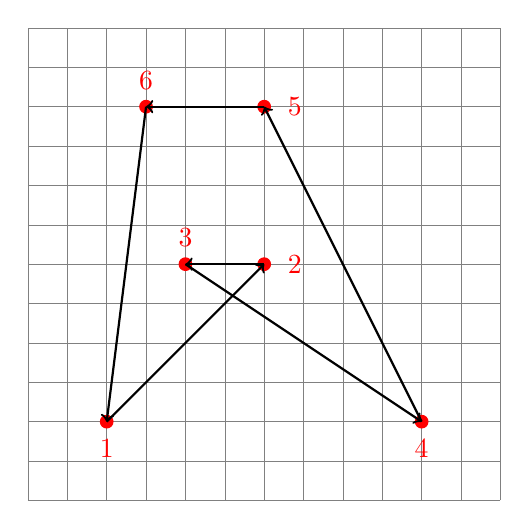
\begin{tikzpicture}
\draw[style=help lines,step=0.5cm] (0,0) grid (6,6);

 \begin{scope}[color=red]
    \filldraw (1,1) circle (0.08cm)  {} node[anchor=north,yshift=-0.1cm] {1};
    \filldraw (3,3) circle (0.08cm) {} node[anchor=west,xshift=5pt] {2};
    \filldraw (2,3) circle (0.08cm){} node[anchor=south,yshift=0.1cm] {3};
    \filldraw (5,1) circle (0.08cm)  {} node[anchor=north,yshift=-0.1cm] {4};
    \filldraw (3,5) circle (0.08cm) {} node[anchor=west,xshift=5pt] {5};
    \filldraw (1.5,5) circle (0.08cm){} node[anchor=south,yshift=0.1cm] {6};
\end{scope}
    
\draw[->,thick] (1,1) -- (3,3);
\draw[->,thick] (3,3) -- (2,3);
\draw[->,thick] (2,3) -- (5,1);
\draw[->,thick] (5,1) -- (3,5);
\draw[->,thick] (3,5) -- (1.5,5);
\draw[->,thick] (1.5,5) -- (1,1);
\end{tikzpicture}
\end{figure}

To detect if the polygon is convex in $O(n)$, we need two satisfy two conditions. First, we must guarantee that all the triples form either only left turns, or only right turns (i.e., maintain the same relative direction). This guarantees that each of the internal angle of the polygon does not exceed 180 degrees. But as shown in the figure, this is not sufficient.

We also need to guarantee that the sum of the internal angles of the polygon is not larger than 360 degrees. For that, we pick the left-bottom-most point $p_b$ ($p_1$ in the figure) and for each point $p_i$ in the polygon, with $i = b+1, b+2, \ldots$, we check if ${CCW}(p_b, p_i, p_i+1)$ is non-negative. That is, the polar angle with respect to $p_b$ should always grow.


\section*{Exercise 5 (10 pts)}

In the online convex hull problem, we are given the set $Q$ of $n$ points one point at a time. After receiving each point, we have to compute the convex hull of the points seen so far. Obviously, we could re-run Graham’s scan every time, yielding a total running time of $O(n^2 \log n)$. Show how to solve the online convex hull problem in $O(n^2)$ time.

\paragraph{Answer.}

\end{document}
